%%%%%%%%%%%%%%%%%%%%%%%%%%%%%%%%%%%%%%%%%%%%%%%%%%%%%%%%%%%%%%%%%%%%%%%%
\chapter{Introduction}
%%%%%%%%%%%%%%%%%%%%%%%%%%%%%%%%%%%%%%%%%%%%%%%%%%%%%%%%%%%%%%%%%%%%%%%%

\begin{center}
  \begin{minipage}{0.5\textwidth}
    \begin{small}
      In which the reasons for doing this Ph.D. are laid bare for the whole world to see and we encounter some answers to questions in which, frankly, only an extremely small number of people were interested in the first place.
    \end{small}
  \end{minipage}
  \vspace{0.5cm}
\end{center}

\noindent This package contains a minimal, modern template for writing your
thesis. While originally meant to be used for a Ph.\,D.\ thesis, you can
equally well use it for your honour thesis, bachelor thesis, and so
on---some adjustments may be necessary, though.

%%%%%%%%%%%%%%%%%%%%%%%%%%%%%%%%%%%%%%%%%%%%%%%%%%%%%%%%%%%%%%%%%%%%%%%%
\section{Goclassy}
%%%%%%%%%%%%%%%%%%%%%%%%%%%%%%%%%%%%%%%%%%%%%%%%%%%%%%%%%%%%%%%%%%%%%%%%

In recent years neural methods for Natural Language Processing (NLP) have consistently and repeatedly improved the state-of-the-art in a wide variety of NLP tasks such as parsing, PoS-tagging, named entity recognition, machine translation, text classification and reading comprehension among others. Probably the main contributing factor in this steady improvement for NLP models is the raise in usage of \emph{transfer learning} techniques in the field. These methods normally consist of taking a pre-trained model and reusing it, with little to no retraining, to solve a different task from the original one it was intended to solve; in other words, one \emph{transfers} the \emph{knowledge} from one task to another.

Most of the transfer learning done in NLP nowadays is done in an unsupervised manner, that is, it normally consists of a  \emph{language model} that is fed unannotated plain text in a particular language; so that it \emph{extracts} or \emph{learns} the basic \emph{features} and patterns of the given language, the model is subsequently used on top of an specialised architecture designed to tackle a particular NLP task. Probably the best known example of this type of model are \emph{word embeddings} which consist of real-valued vector representations that are trained for each word on a given corpus. Some notorious examples of word embeddings are word2vec \citep{mikolov-etal-2013-distributed}, GloVe \citep{pennington-etal-2014-glove} and \mbox{fastText} \citep{mikolov-etal-2018-advances}. All these models are \emph{context-free}, meaning that a given word has one single vector representation that is independent of context, thus for a polysemous word like Washington, one would have one single representation that is reused for the city, the state and the US president.

In order to overcome the problem of polysemy, \emph{contextual} models have recently appeared. Most notably ELMo \citep{peters-etal-2018-deep} which produces deep contextualised word representations out of the internal states of a deep bidirectional language model in order to model word use and how the usage varies across linguistic contexts. ELMo still needs to be used alongside a specialised architecture for each given downstream task, but newer architectures that can be fine-tuned have also appear. For these, the model is first fed unannotated data, and is then fine-tuned with annotated data to a particular downstream task without relying on any other architecture. The most remarkable examples of this type of model are GPT-1, GPT-2 \citep{radford-etal-2018-improving,radford-etal-2019-language}, BERT \citep{devlin-etal-2019-bert} and XLNet \citep{yang-etal-2019-xlnet}; the latter being the current state-of-the-art for multiple downstream tasks. All of these models are different arrangements of the Transformer architecture \citep{vaswani-etal-2017-attention} trained with different datasets, except for XLNet which is an instance of the Transformer-XL \citep{dai-etal-2019-transformer}.

Even though these models have clear advantages, their main drawback is the amount of data that is needed to train them in order to obtain a functional and efficient model. For the first English version of word2vec, \citet{mikolov-etal-2013-distributed} used a one billion word dataset consisting of various news articles. Later \citet{al-rfou-etal-2013-polyglot} and then \citet{bojanowski-etal-2017-enriching} used the plain text from Wikipedia to train distributions of word2vec and fastText respectively, for languages other than English. Now, the problem of obtaining large quantities of data aggravates even more for contextual models, as they normally need multiple instances of a given word in order to capture all its different uses and in order to avoid overfitting due to the large quantity of hyperparameters that these models have. \citet{peters-etal-2018-deep} for example use a 5.5 billion token\footnote{Punctuation marks are counted as tokens.} dataset comprised of crawled news articles plus the English Wikipedia in order to train ELMo, \citet{devlin-etal-2019-bert} use a 3.3 billion word\footnote{Space sparated tokens.} corpus made by merging the English Wikipedia with the BooksCorpus \citep{zhu-etal-2015-aligning}, and \citet{radford-etal-2019-language} use a 40GB English corpus created by scraping outbound links from Reddit.\footnote{\url{https://www.reddit.com/}}

While Wikipedia is freely available, and multiple pipelines exist\footnote{\url{https://github.com/attardi/wikiextractor}}\textsuperscript{,}\footnote{\url{https://github.com/hghodrati/wikifil}} to extract plain text from it, some of the bigger corpora mentioned above are not made available by the authors either due to copyright issues or probably because of the infrastructure needed to serve and distribute such big corpora. Moreover the vast majority of both these models and the corpora they are trained with are in English, meaning that the availability of high quality NLP for other languages, specially for low-resource languages, is rather limited.

%%%%%%%%%%%%%%%%%%%%%%%%%%%%%%%%%%%%%%%%%%%%%%%%%%%%%%%%%%%%%%%%%%%%%%%%
\section{Monolingual approach}
%%%%%%%%%%%%%%%%%%%%%%%%%%%%%%%%%%%%%%%%%%%%%%%%%%%%%%%%%%%%%%%%%%%%%%%%

One of the key elements that has pushed the state of the art considerably in neural NLP in recent years has been the introduction and spread of transfer learning methods to the field. These methods can normally be classified in two categories according to how they are used:
\begin{itemize}
    \item \emph{Feature-based} methods, which involve pre-training real-valued vectors (``embeddings'') at the word, sentence, or paragraph level; and using them in conjunction with a specific architecture for each individual downstream task.
    \item \emph{Fine-tuning} methods, which introduce a minimal number of task-specific parameters, and instead copy the weights from a pre-trained network and then tune them to a particular downstream task.
\end{itemize}
Embeddings or language models can be divided into \emph{fixed}, meaning that they generate a single representation for each word in the vocabulary; and \emph{contextualized}, meaning that a representation is generated based on both the word and its surrounding context, so that a single word can have multiple representations, each one depending on how it is used.

In practice, most fixed embeddings are used as feature-based models. The most notable examples are \emph{word2vec} \citep{mikolov-etal-2013-distributed}, \emph{GloVe} \citep{pennington-etal-2014-glove} and \emph{fastText} \citep{mikolov-etal-2018-advances}. All of them are extensively used in a variety of applications nowadays. On the other hand, contextualized word representations and language models have been developed using both feature-based architectures, the most notable examples being ELMo and Flair \citep{peters-etal-2018-deep,akbik-etal-2018-contextual}, and transformer based architectures, that are commonly used in a fine-tune setting, as is the case of GPT-1, GPT-2 \citep{radford-etal-2018-improving,radford-etal-2019-language}, BERT and its derivatives \citep{devlin-etal-2019-bert,liu-etal-2019-roberta,lan-etal-2020-albert} and more recently T5 \citep{raffel-etal-2020-exploring}. All of them have repeatedly improved the state-of-the art in many downstream NLP tasks over the last year.

In general, the main advantage of using language models is that they are mostly built in an \emph{unsupervised} manner and they can be trained with raw, unannotated plain text. Their main drawback is that enormous quantities of data seem to be required to properly train them especially in the case of contextualized models, for which larger corpora are thought to be needed to properly address polysemy and cover the wide range of uses that commonly exist within languages.

For gathering data in a wide range of languages, Wikipedia is a commonly used option. It has been used to train fixed embeddings \citep{al-rfou-etal-2013-polyglot,bojanowski-etal-2017-enriching} and more recently the multilingual BERT \citep{devlin-etal-2019-bert}, hereafter mBERT. However, for some languages, Wikipedia might not be large enough to train good quality contextualized word embeddings. Moreover, Wikipedia data all belong to the same specific genre and style. To address this problem, one can resort to crawled text from the internet; the largest and most widespread dataset of crawled text being Common Crawl.\footnote{\url{https://commoncrawl.org}} Such an approach generally solves the quantity and genre/style coverage problems but might introduce noise in the data, an issue which has earned the corpus some criticism, most notably by \citet{trinh-le-2018-a} and \citet{radford-etal-2019-language}. Using Common Crawl also leads to data management challenges as the corpus is distributed in the form of a large set of plain text each containing a large quantity of unclassified multilingual documents from different websites.

%%%%%%%%%%%%%%%%%%%%%%%%%%%%%%%%%%%%%%%%%%%%%%%%%%%%%%%%%%%%%%%%%%%%%%%%
\section{Quality at Glance}
%%%%%%%%%%%%%%%%%%%%%%%%%%%%%%%%%%%%%%%%%%%%%%%%%%%%%%%%%%%%%%%%%%%%%%%%

Access to multilingual datasets for NLP research has vastly improved over the past years. A variety of web-derived collections for hundreds of languages is available for anyone to download, such as ParaCrawl~\citep{espla-etal-2019-paracrawl, banon-etal-2020-paracrawl}, WikiMatrix~\citep{schwenk-etal-2021-wikimatrix} CCAligned~\citep{el-kishky-etal-2020-ccaligned}, \mbox{OSCAR}~\citep{ortiz-suarez-etal-2019-asynchronous, ortiz-suarez-etal-2020-monolingual}, and several others.
These have in turn enabled a variety of highly multilingual models, like mT5 \citep{xue-etal-2021-mt5}, M2M\nobreakdash-100 \citep{fan-etal-2020-beyond}, M4 \citep{arivazhagan-etal-2019-massively}.
% Recent approaches that employ large-scale multilingual systems have shown potential for some generalization across typologically different languages \cite{pires-etal-2019-multilingual,papadimitriou-etal-2021-deep}. .

Curating such datasets relies on the websites giving clues about the language of their contents (e.g. a language identifier in the URL) and on automatic language classification (LangID).
%and filtering tools, and a range of evaluation sets and metrics to compile high-quality datasets. 
It is commonly known that these automatically crawled and filtered datasets tend to have overall lower quality than hand-curated collections~\citep{koehn-etal-2020-findings}, but their quality is rarely measured directly, and is rather judged through the improvements they bring to downstream applications~\citep{schwenk-etal-2021-wikimatrix}.

Building NLP technologies with automatically crawled datasets is promising. This is especially true for low-resource languages, because data scarcity is one of the major bottlenecks for deep learning approaches.
However, there is a problem: There exists very little research on evaluating both data collections and automatic crawling and filtering tools for low-resource languages.
As a result, although many low-resource languages are covered by the latest multilingual crawl data releases, their quality and thus usability is unknown.


%%%%%%%%%%%%%%%%%%%%%%%%%%%%%%%%%%%%%%%%%%%%%%%%%%%%%%%%%%%%%%%%%%%%%%%%
\section{Towards}
%%%%%%%%%%%%%%%%%%%%%%%%%%%%%%%%%%%%%%%%%%%%%%%%%%%%%%%%%%%%%%%%%%%%%%%%

The demand for large corpora has considerably increased in recent years with the advent of semi-supervised learning methods in Natural Language Processing (NLP), such as \emph{word embeddings} \cite{mikolov-etal-2013-distributed,pennington-etal-2014-glove,mikolov-etal-2018-advances}, \emph{contextualized word representations} \cite{howard-ruder-2018-universal,peters-etal-2018-deep,devlin-etal-2019-bert} and more recently \emph{very large generative language models} like GPT-3, T5, GPT-Neo \cite{raffel-etal-2020-exploring,brown-etal-2020-language,black-etal-2021-gpt}. While there have been some recent efforts to manually curate such corpora\footnote{\url{https://bigscience.huggingface.co}} \cite{gao-etal-2020-pile}, the common approach to collect large amounts of raw textual data still relies primarily on crawled web text \cite{ortiz-suarez-etal-2019-asynchronous,ortiz-suarez-etal-2020-monolingual,xue-etal-2021-mt5,el-kishky-etal-2020-ccaligned,espla-etal-2019-paracrawl,banon-etal-2020-paracrawl,gao-etal-2020-pile}, and although some of the initial concerns of using crawled data \cite{trinh-le-2018-a,radford-etal-2019-language} have been addressed in recent years \cite{ortiz-suarez-etal-2020-monolingual,martin-etal-2020-camembert} there a many concerns that still need to be tackled \cite{caswell-etal-2020-language} specially for multilingual data \cite{kreutzer-etal-2021-quality}.

In this demand for large raw textual corpora we can observe a clear back and forth in the type of data used to pre-train these models. On one hand some authors have opted for highly curated or edited data like Wikipedia such as \newcite{al-rfou-etal-2013-polyglot} and \newcite{bojanowski-etal-2017-enriching} for static word embeddings, the 1B Word Benchmark \cite{chelba-etal-2014-one} for ELMo \cite{peters-etal-2018-deep}, and the BookCorpus \cite{zhu-etal-2015-aligning} and Wikipedia for BERT \cite{devlin-etal-2019-bert}. On the other hand projects like those of \newcite{pennington-etal-2014-glove} or \newcite{grave-etal-2018-learning} used crawled data for the pre-training of fixed word embeddings, CamemBERT \cite{martin-etal-2020-camembert} a contextualized model for French successfully used only Crawled data for pre-training, and even large generative language models like T5 have used mainly crawled data successfully \cite{raffel-etal-2020-exploring}. We can of course also see examples of projects successfully using a mix of both manually curated and automatically crawled data such as RoBERTa \cite{liu-etal-2019-roberta}, XLNet \cite{yang-etal-2019-xlnet} and GPT-Neo \cite{black-etal-2021-gpt,gao-etal-2020-pile}. However, no matter the chosen approach to build these large corpora, there are in every case concerns that have been expressed, specially for the datasets used in very large generative language models \cite{bender-etal-2021-on}, even when using manually edited resources like Wikipedia \cite{barera-2020-mind}.


%%%%%%%%%%%%%%%%%%%%%%%%%%%%%%%%%%%%%%%%%%%%%%%%%%%%%%%%%%%%%%%%%%%%%%%%
\section{CamemBERT}
%%%%%%%%%%%%%%%%%%%%%%%%%%%%%%%%%%%%%%%%%%%%%%%%%%%%%%%%%%%%%%%%%%%%%%%%

Pretrained word representations have a long history in Natural Language Processing (NLP), from non-contextual \citep{brown-etal-1992-class,ando-zhang-2005-framework,mikolov-etal-2013-distributed,pennington-etal-2014-glove} to contextual word embeddings \citep{peters-etal-2018-deep,akbik-etal-2018-contextual}. Word representations are usually obtained by training language model architectures on large amounts of textual data and then fed as an input to more complex task-specific architectures. More recently, these specialized architectures have been replaced altogether by large-scale pretrained language models which are \emph{fine-tuned} for each application considered. This shift has resulted in large improvements in performance over a wide range of tasks \cite{devlin-etal-2019-bert,radford-etal-2019-language,liu-etal-2019-roberta,raffel-etal-2020-exploring}.

These transfer learning methods exhibit clear advantages over more traditional task-specific approaches. In particular, they can be trained in an \emph{unsupervized} manner, thereby taking advantage of the information contained in large amounts of raw text.
Yet they come with implementation challenges, namely the amount of data and computational resources needed for pre-training, which can reach hundreds of gigabytes of text and require hundreds of GPUs \citep{yang-etal-2019-xlnet,liu-etal-2019-roberta}. This has limited the availability of these state-of-the-art models to the English language, at least in the monolingual setting. This is particularly inconvenient as it hinders their practical use in NLP systems. It also prevents us from investigating their language modelling capacity, for instance in the case of morphologically rich languages.

%%%%%%%%%%%%%%%%%%%%%%%%%%%%%%%%%%%%%%%%%%%%%%%%%%%%%%%%%%%%%%%%%%%%%%%%
\section{FrELMo}
%%%%%%%%%%%%%%%%%%%%%%%%%%%%%%%%%%%%%%%%%%%%%%%%%%%%%%%%%%%%%%%%%%%%%%%%
\label{sec:intro}

Named entity recognition (NER) is the widely studied task consisting in identifying text spans that denote \emph{named entities} such as person, location and organization names, to name the most important types. Such text spans are called named entity \emph{mentions}. In NER, mentions are generally not only identified, but also classified according to a more or less fine-grained ontology, thereby allowing for instance to distinguish between the telecommunication company \emph{Orange} and the town \emph{Orange} in southern France (amongst others). Importantly, it has long been recognised that the type of named entities can be defined in two ways, which underlies the notion of metonymy: the intrinsic type (\emph{France} is always a location) and the contextual type (in \emph{la France a signé un traité} `France signed a treaty', \emph{France} denotes an organization).


NER has been an important task in natural language processing for quite some time. It was already the focus of the MUC conferences and associated shared tasks
\cite{marsh-perzanowski-1998-muc}, and later that of the CoNLL~2003 and ACE shared tasks \cite{tjong-kim-sang-de-meulder-2003-introduction,doddington-etal-2004-automatic}. Traditionally, as for instance was the case for the MUC shared tasks, only person names, location names, organization names, and sometimes ``other proper names'' are considered. However, the notion of named entity mention is sometimes extended to cover any text span that does not follow the general grammar of the language at hand, but a type- and often culture-specific grammar, thereby including entities ranging from product and brand names to dates and from URLs to monetary amounts and other types of numbers.

As for many other tasks, NER was first addressed using rule-based approaches, followed by statistical and now neural machine learning techniques (see Section~\ref{subsec:sota} for a brief discussion on NER approaches). Of course, evaluating NER systems as well as training machine-learning-based NER systems, statistical or neural, require named-entity-annotated corpora.
Unfortunately, most named entity annotated French corpora are oral transcripts, and they are not always freely available. The ESTER and ESTER2 corpora (60 plus 150 hours of NER-annotated broadcast transcripts)
\cite{galliano-etal-2005-the,galliano-etal-2009-the}, as well as the Quaero
\cite{grouin-etal-2011-proposal} corpus are based on oral transcripts (radio broadcasts). Interestingly, the Quaero corpus relies on an original, very rich and structured  definition of the notion of named entity \cite{rosset-etal-2011-entites}. It contains both the intrinsic and the contextual types of each mention, whereas the ESTER and ESTER2 corpora only provide the contextual type.

%%%%%%%%%%%%%%%%%%%%%%%%%%%%%%%%%%%%%%%%%%%%%%%%%%%%%%%%%%%%%%%%%%%%%%%%
\section{SinNER}
%%%%%%%%%%%%%%%%%%%%%%%%%%%%%%%%%%%%%%%%%%%%%%%%%%%%%%%%%%%%%%%%%%%%%%%%

Among the aspects for which Natural Language Processing (NLP) can be useful for Digital Humanities (DH) figures prominently Named Entity Recognition. This task interests researchers for numerous reasons since the application can be pretty wide.
We can cite genealogy or history for which finding mentions of persons and places in texts is very useful. Researchers in digital literature have shown a great interest in NER since it can help for instance to highlight the path of different characters in a book or in a book series. There can be cross-fertilization between NER and DH since some researchers showed that some particular properties of literature can help to build better NER systems \cite{brooke-etal-2016-bootstrapped}.
Apart from literature, NER can also be used more generally to help refine queries to assist browsing in newspaper collections \cite{neudecker-etal-2014-large}.
Like other NLP tasks, NER quality will suffer from different problems related to variations in the input data: variation in languages (multilinguality), variation in the quality of the data (OCR errors mainly) and specificity of the application domain (literature vs. epidemic surveillance for instance). These difficulties can be connected with the challenges for low-level NLP tasks highlighted by Dale \textit{et al.} \cite{dale-etal-2000-handbook}. In CLEF-HIPE shared task \cite{ehrmann-etal-2020-extended}, the variation in language and in text quality will be the main problems even if the specificity of the application can be of great interest.

NER in old documents represent an interesting challenge for NLP since it is usually necessary to process documents that show different kind of variations as compared to the particular laboratory conditions on which NER systems are trained.
Most NER systems are usually designed to process clean data.
Additionally, there is the multilingual issue since NER systems have been designed primarily for English, with assumptions on the availability of data on the one hand and on the universal nature of some linguistic properties on the other hand.

The fact that the texts processed in Digital Humanities are usually not born-digital is very important since, even after OCR post-correction, it is very likely that some noise would be found in the text.
Other difficulties will arise as well in those type of documents. The variation in language is one of them since contemporary English will clearly not be the most frequent language.  It is interesting for researchers to check how much diachronic variation has an influence on NER systems \cite{ehrmann-etal-2016-diachronic}.
It makes it even more important to work on multilingual NER and to build architectures that need less training data \cite{rahimi-etal-2019-massively}.
More generally, NER in ancient texts represents a great opportunity for NLP to compare to main approaches to handle variation in texts: adapting the texts to an existing architecture via modernization or normalization \cite{leaman-etal-2016-taggerone} or adapting the pipeline to non standard data (OCR noise, language variants\dots) via domain adaptation or data augmentation techniques \cite{ghannay-etal-2018-end}.


%%%%%%%%%%%%%%%%%%%%%%%%%%%%%%%%%%%%%%%%%%%%%%%%%%%%%%%%%%%%%%%%%%%%%%%%
\section{BERTrade}
%%%%%%%%%%%%%%%%%%%%%%%%%%%%%%%%%%%%%%%%%%%%%%%%%%%%%%%%%%%%%%%%%%%%%%%%

% Context
There is a growing interest in digital humanities for automatic processing and annotation of historical texts. In this work, we study how to take advantage of current NLP models of the BERT family to advance the state of the art in processing historical languages, taking Old French (9th-13th century French) as a use case.

Old French is one of the historical languages for which we have the largest amount of syntactically annotated data, and we expect that our results on these language states may be generalised and used as a source of inspiration for researchers currently developing annotated resources for other historical languages.

Using contextual word embeddings as input representations has brought clear gains in performances for most of the NLP tasks for which they have been used.
However, this has mostly been attested in languages where sufficient (raw) linguistic data is available.
For less-resourced languages, the most common approach has been to leverage multilingual models such as mBERT \citep{devlin-etal-2019-bert}

Historical languages are typical cases where available linguistic data is limited, with no chance of acquiring new texts. They are also not normalized by spelling and institutional conventions and tend to be more heterogeneous than contemporary lesser-resourced languages.

\subsection{Medeival French}

\begin{figure}[thb]
  \centering
  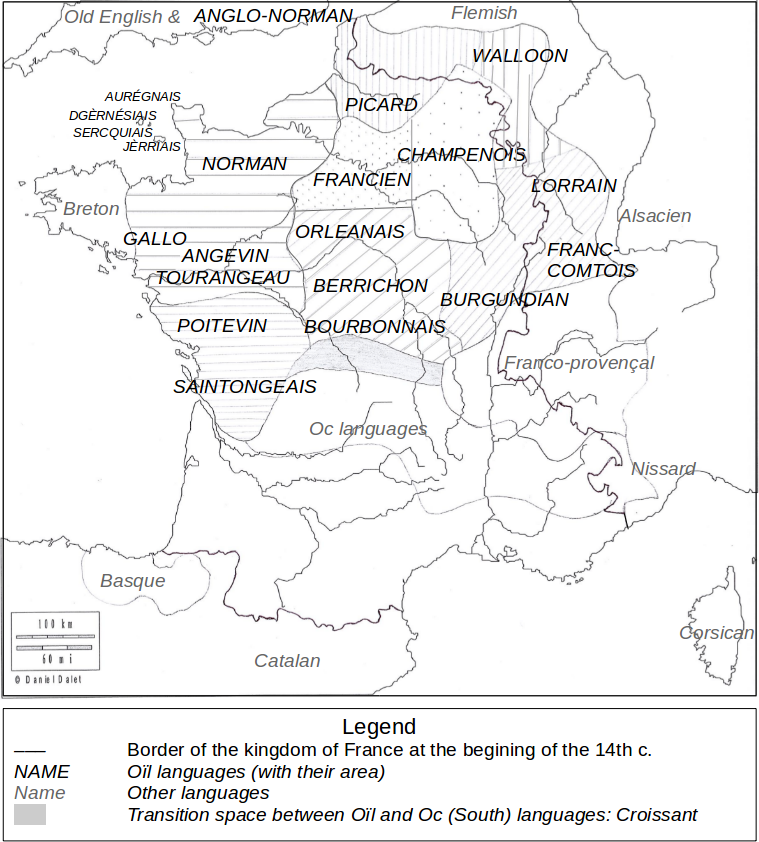
\includegraphics[scale=0.29]{static/media/mod_eval/bertrade/map-dialects2.png}
  \caption{Oïl languages}
  \label{fig:map-dialects}
\end{figure}

Medieval French covers both Old French (9th-13th c.) and Middle French (14th-15th c.). These stages are linguistically close and both precede the adoption of spelling norms. Middle French is more regular than Old French in some respects such as word order \citep{marchello-Nizia-etal-2020-grande} and less in others such as NP structure and pronouns system \citep{marchello-nizia-etal-1979-histoire}. Medieval French covers a set of \textit{Oïl} Romance languages spoken in the kingdom of France between the 9th and the 15th century (\cref{fig:map-dialects}).
There are around twenty such languages.

Older texts are close to Late Latin, and verse is prevalent until the end of the 13th century. Old French has a relatively free word order.
Until the mid-11th century, the prevalent order is \textit{Subject-Object-Verb} (SOV), which is then gradually supplanted by SVO, which is the default order in contemporary French. Unlike most languages with free word order, the functions of verbal arguments are not always given away by morphological clues, the already simplistic case system of Old French disappears progressively through the covered period.

There are also many cases of syntactic ambiguity. For example, in the following quote from \emph{Lancelot},\footnote{In the edition from Pierre Kunstmann, from the online \textit{Base de français médiéval}: \url{http://catalog.bfm-corpus.org/CharretteKu}.} (verse ~5436),
both \enquote{la dame} and \enquote{Lancelot} could be the subject or the object of \enquote{Vit} and only the context enables the reader to understand that \enquote{la dame} is the subject.

\digloss{Dolant et pansif Lancelot Vit la dame}
{Mournful and meditative Lancelot saw the lady}
{The lady saw that Lancelot was mournful and meditative.}

Word order is also relatively free within constituents. For example, a noun modifier can be on the left or on the right of its governor, and it is not necessarily preceded by a preposition. In contemporary French, it can only appear on the right, and it is found without a preposition only in some cases like named entities. Because of the general free word order and the absence of punctuation in our treebank, this adds up to the ambiguity of the analysis.

In each of the following examples from the SRCMF corpus, the noun following \emph{roi} (\enquote{king}) has a different analysis: head of \emph{roi}, modifier, argument of the same verb or a different one, with no explicit marking:

\begin{center}
    % beroul. modifieur à gauche.
    \begin{dependency}[theme=simple]
        \begin{deptext}[row 2/.style={font=\small}]
            \textit{Fus} \& \textit{tu} \& \textit{donc} \& \textit{pus} \& \textit{a} \& \textit{la} \& \textbf{\textit{roi}} \& \textit{cort} \\
            %VERB \& PRON \& ADV \& ADV \& ADP \& DET \& NOUN \& NOUN \\
            Were \& you \& then \& no more \& at \& the \& king \& court \\
        \end{deptext}
        \depedge{8}{7}{nmod}
        \depedge[edge start x offset=0.5em]{8}{6}{det}
        \depedge[edge start x offset=1em]{8}{5}{case}
    \end{dependency}

    \raggedright
    \enquote{Then were you not at the king's court anymore?} (\emph{Beroul Tristan})
\end{center}

\begin{center}
    % Graal. modifieur à droite.
    \begin{dependency}[theme=simple]
        \begin{deptext}[row 2/.style={font=\small}]
            \textit{la} \& \textit{fille} \& \textit{au} \& \textit{riche} \& \textbf{\textit{roi}} \& \textit{pescheor} \\
            the \& daughter \& of the \& rich \& king \& fisher \\
        \end{deptext}
        \depedge{5}{6}{flat}
    \end{dependency}

    \raggedright
    \enquote{the daughter of the rich Fisher King} (\emph{Queste del Saint Graal})
\end{center}

\begin{center}
    % Roland. arguments du même verbe.
    \begin{dependency}[theme=simple]
        \begin{deptext}[row 2/.style={font=\small}]
            \textit{De} \& \textit{Guenelun} \& \textit{atent} \& \textit{li} \& \textbf{\textit{reis}} \& \textit{nuveles} \\
            From \& Ganelon \& waits \& the \& king \& news \\
        \end{deptext}
        \depedge{3}{5}{nsubj}
        \depedge[edge start x offset=-0.5em]{3}{6}{obj}
    \end{dependency}

    \raggedright
    \enquote{The king waits for news from Ganelon.} (\emph{Chanson de Roland})
\end{center}

\begin{center}
    % Graal. arguments de verbes différents, et absence de ponctuation.
    \begin{dependency}[theme=simple]
        \begin{deptext}[row 2/.style={font=\small}]
            \textit{Biax} \& \textit{sire} \& \textit{fet} \& \textit{li} \& \textbf{\textit{rois}} \& \textit{escu} \& \textit{vos} \& \textit{envoiera} \& \textit{Diex} \\
            Dear \& Sir \& says \& the \& king \& shield \& you \& send-FUT \& God \\
        \end{deptext}
        \depedge{3}{5}{nsubj}
        \depedge{8}{6}{obj}
    \end{dependency}

    \raggedright
    \enquote{Dear Sir, says the king, God will send you a shield.} (\emph{Queste del Saint Graal})
\end{center}

Furthermore, overt subjects are not mandatory, and are often dropped in texts written in verse until the 12th century, after which the presence of subjects increases through time.
These phenomena are particularly prevalent in verse, where metric and rhyming constraints often lead to more contrived syntactic forms than in prose.

Another source of ambiguity is the variety of spellings, due to the lack of spelling standard. For example, the word \textit{moult} (transl. \textit{a lot (of), very}), emblematic of this period, is initially an adjective, and it is progressively grammaticalized, becoming an adverb. Several forms appear at the same time, some with a declension, some without, and the radical does not have a fixed spelling: \textit{molt(e)(s), molz, mult(e)(s), mul(t)z, mou(l)t}…

%%%%%%%%%%%%%%%%%%%%%%%%%%%%%%%%%%%%%%%%%%%%%%%%%%%%%%%%%%%%%%%%%%%%%%%%
\section{D'AlemBERT}
%%%%%%%%%%%%%%%%%%%%%%%%%%%%%%%%%%%%%%%%%%%%%%%%%%%%%%%%%%%%%%%%%%%%%%%%

With the rise of digital humanities, it is becoming increasingly important to develop high quality tools to automatically process old states of languages. Libraries, archives and museums, among others, are digitising large numbers of historical sources, from which high quality data must be extracted for further study by specialists of human sciences following new approaches such as ``distant reading'' \cite{moretti-2013-distant}. Many (sub)tasks such as automatic OCR post-correction \cite{rijhwani-etal-2021-lexically} and linguistic annotation \cite{camps-etal-2021-corpus} benefit from pretrained language models to improve their accuracy, and this is what motivated us to develop a BERT-like \cite{devlin-etal-2019-bert} contextualised language model for Early Modern French.

Languages evolve over time on many different levels: from one century to another, we see variations in spelling, syntax, the lexicon etc. However this variation is not uniform: it tends, at least for ``literate scriptors'' (literature, journalism, law, etc.), to converge towards a single norm over time, and this has especially been the case for French because of the prominent role of the \emph{Académie française} and the \emph{remarqueurs} \cite{ayres-bennett-etal-2011-remarques}. The result of this convergence is, for instance, that spelling and word order within sentences have become more strict, where they were less so in the past. From a computational perspective, historical states of language are therefore not only different from the contemporary state, but, from a computational perspective, are also more complex because they do not follow a strict and explicit norm. In French, this explicit norm  appeared in the 17\textsuperscript{th}~c. and was slowly integrated throughout the 18\textsuperscript{th}~c.

On top of this first linguistic problem, a second issue appears: because the production of textual sources has continued to grow exponentially, it is easier to collect a corpus for contemporary French  than for the 19\textsuperscript{th}\,c. French, which is itself easier than for the 18\textsuperscript{th}\,c. French, etc. The further we go back in time, the more scarce resources are, which creates the following paradox: we have more data when the language is homogeneous and simple for the computer to process, and less when it is heterogeneous and harder to process.

\subsection{Early Modern French}\label{def:early}

\begin{table*}[!htp]
    \centering\small
    \begin{tabular}{@{}p{0.3\linewidth}p{0.3\linewidth}p{0.3\linewidth}@{}}
        \toprule
        Source                                                                                                                                                                                                                                                                                               & Normalised & Translation \\
        \midrule
        Surquoy, SIRE, s’il plaiſt à voſtre Maieſté de ſe ſouuenir des miſeres de ſon Eſtat, dõt au moins ell’a tiré cét aduantage, qu’en vne grande ieuneſse ell’a acquis vne grande experi\~ece, elle verra que tous les mal-heurs de sõ bas âge ont pris leur commencement en ſemblables occaſions;       &
        \emph{Sur quoi, SIRE, s’il plaît à votre Majesté de se souvenir des misères de son état dont au moins elle a tiré cet avantage, qu’en une grande jeunesse elle a acquis une grande expérience, elle verra que tous les malheurs de son bas âge ont pris leur commencement en semblables occasions~;} &
        \textcolor{gray}{``Whereupon, SIR, if it pleases your Majesty to remember the miseries of her state, from which at least she has derived this advantage, that in great youth she has acquired great experience, she will see that all the misfortunes of her early life took their beginning on similar occasions;''}           \\
        \bottomrule
    \end{tabular}
    \caption{\label{tab:norm_examples}Example of normalisation taken from the \emph{Lettres} of \protect\newcite{balzac-1624-lettres}.}
\end{table*}

We loosely define Early Modern French as a state of language following Middle French in 1500---following here the \emph{terminus ad quem} used by the \emph{Dictionnaire de Moyen Français} \cite{martin-2020-dictionnaire}---and ending with the French Revolution in 1789. It therefore encompasses three centuries (16\textsuperscript{th}, 17\textsuperscript{th} and 18\textsuperscript{th}\,c.), or two linguistic periods: the \emph{français préclassique} or ``preclassical French'', 1500--1630 and the \emph{français classique} or ``classical French'', 1630--1689; both periodisations are currently used in French linguistics (\emph{e.g.}~by \newcite{vachon-2010-changement} and \newcite{amatuzzi-etal-2019-ameliorer}).

A typical example of Early Modern French, taken from ~\newcite{balzac-1624-lettres}, is given in Table~\ref{tab:norm_examples}. We note here the presence of several phenomena that have now disappeared in contemporary French, such as the presence of abbreviations (\emph{dõt}$\to$\emph{dont}), the long \emph{s} (\emph{ſ}, see\,\emph{miſeres}), the use of \emph{v} instead of \emph{u} (\emph{vne} for \emph{une}), the conservation of etymological letters (\emph{voſtre}$<$Latin~\emph{vŏster} rather than \emph{votre}) and calligraphic letters (\emph{-y} in \emph{Surquoy}), the absence of welding  (\emph{\mbox{mal-heurs}} and not \emph{malheurs}) and the opposite (\emph{Surquoy} and not \emph{Sur quoi}).

For NLP tasks, which process raw sequences, such differences with respect to contemporary French are not trivial, and they prevent the processing of historical texts with tools trained on recent sources.